\documentclass[conference]{IEEEtran}

\usepackage{cite}
\usepackage{amsmath,amssymb,amsfonts}
\usepackage{algorithm}
\usepackage{algorithmic}
\usepackage{graphicx}
\usepackage{textcomp}
\usepackage{xcolor}
\def\BibTeX{{\rm B\kern-.05em{\sc i\kern-.025em b}\kern-.08em
    T\kern-.1667em\lower.7ex\hbox{E}\kern-.125emX}}
\begin{document}

\title{Ray Tracing In Functional Programming Language\\

}

\author{\IEEEauthorblockN{Dr. Babul Prasad Tewari}
\IEEEauthorblockA{\textit{Department of} \\
\textit{ Computer Science and Engineering}\\
\textit{GKCIET}\\
Malda, India \\
babul@gkciet.ac.in}
\and
\IEEEauthorblockN{Aditya Raj}
\IEEEauthorblockA{\textit{Department of} \\
\textit{ Computer Science and Engineering}\\
\textit{GKCIET}\\
Malda, India \\
induaditya214@gmail.com}
\and
\IEEEauthorblockN{3\textsuperscript{rd} Given Name Surname}
\IEEEauthorblockA{\textit{dept. name of organization (of Aff.)} \\
\textit{name of organization (of Aff.)}\\
City, Country \\
email address or ORCID}
}

\maketitle

\begin{abstract}
to do
\end{abstract}

\begin{IEEEkeywords}
ray tracing, three-dimensional graphics, functional programming.
\end{IEEEkeywords}

\section{Introduction}

There are two approaches to rendering a three-dimensional scene: object-order rendering and image-order rendering. 

Object-order rendering involves iterating over each object and figuring out which set of pixels it maps to and coloring those pixels.
In image-order rendering, for each pixel, the nearest visible object is found, and that pixel is colored using the given shading model. 
The former is classified into rasterization algorithms (or projective algorithms), and the latter is termed the ray tracing algorithm (image-space algorithm). Same effects, like reflections and shadows, are easy to implement in ray tracing compared to rasterization.

In ray tracing, image synthesis happens by shooting rays that go through the projection plane, and the nearest intersection with an object is found. If the object is reflective, rays bounce off it and hit other objects, which also influences color according to the shading model. In the current implementation, we have utilized the simplest shading model called Blinn-Phong shading and used the simplest three-dimensional geometrical object, a sphere, to illustrate ray tracing in the functional programming paradigm. To this end, we decided to use OCaml for its strong support for functional programming and its mechanisms to write imperative code as well, which will enable us to demonstrate alternative ways in the same programming language.
\section{Methodlogy}

\begin{algorithm}
    \caption{Ray Tracing Algorithm}
    \begin{algorithmic}[1]
        \STATE Initialize scene with objects and lights
        \STATE Set canvas resolution (width, height)
        \STATE For each pixel (x, y) in the canvas:
            \STATE \quad Generate ray from camera through pixel (x, y)
            \STATE \quad Initialize color to background color
            \STATE \quad Initialize closest intersection distance to infinity
            \STATE \quad For each object in the scene:
                \STATE \quad \quad If ray intersects object:
                    \STATE \quad \quad \quad Calculate intersection point
                    \STATE \quad \quad \quad Calculate normal at intersection point
                    \STATE \quad \quad \quad Calculate distance to intersection
                    \STATE \quad \quad \quad If distance is less than closest intersection distance:
                        \STATE \quad \quad \quad \quad Update closest intersection distance
                        \STATE \quad \quad \quad \quad Calculate color at intersection point
                        \STATE \quad \quad \quad \quad Update color based on lighting
            \STATE \quad Set pixel color to calculated color
        \STATE Render the image
    \end{algorithmic}
\end{algorithm}
 
\subsection{Blinn-Phong Shading Model}


\subsection{Equations}
to do
\begin{equation}
a+b=\gamma\label{eq}
\end{equation}



``Fig.~\ref{fig}''



\begin{figure}[htbp]
\centerline{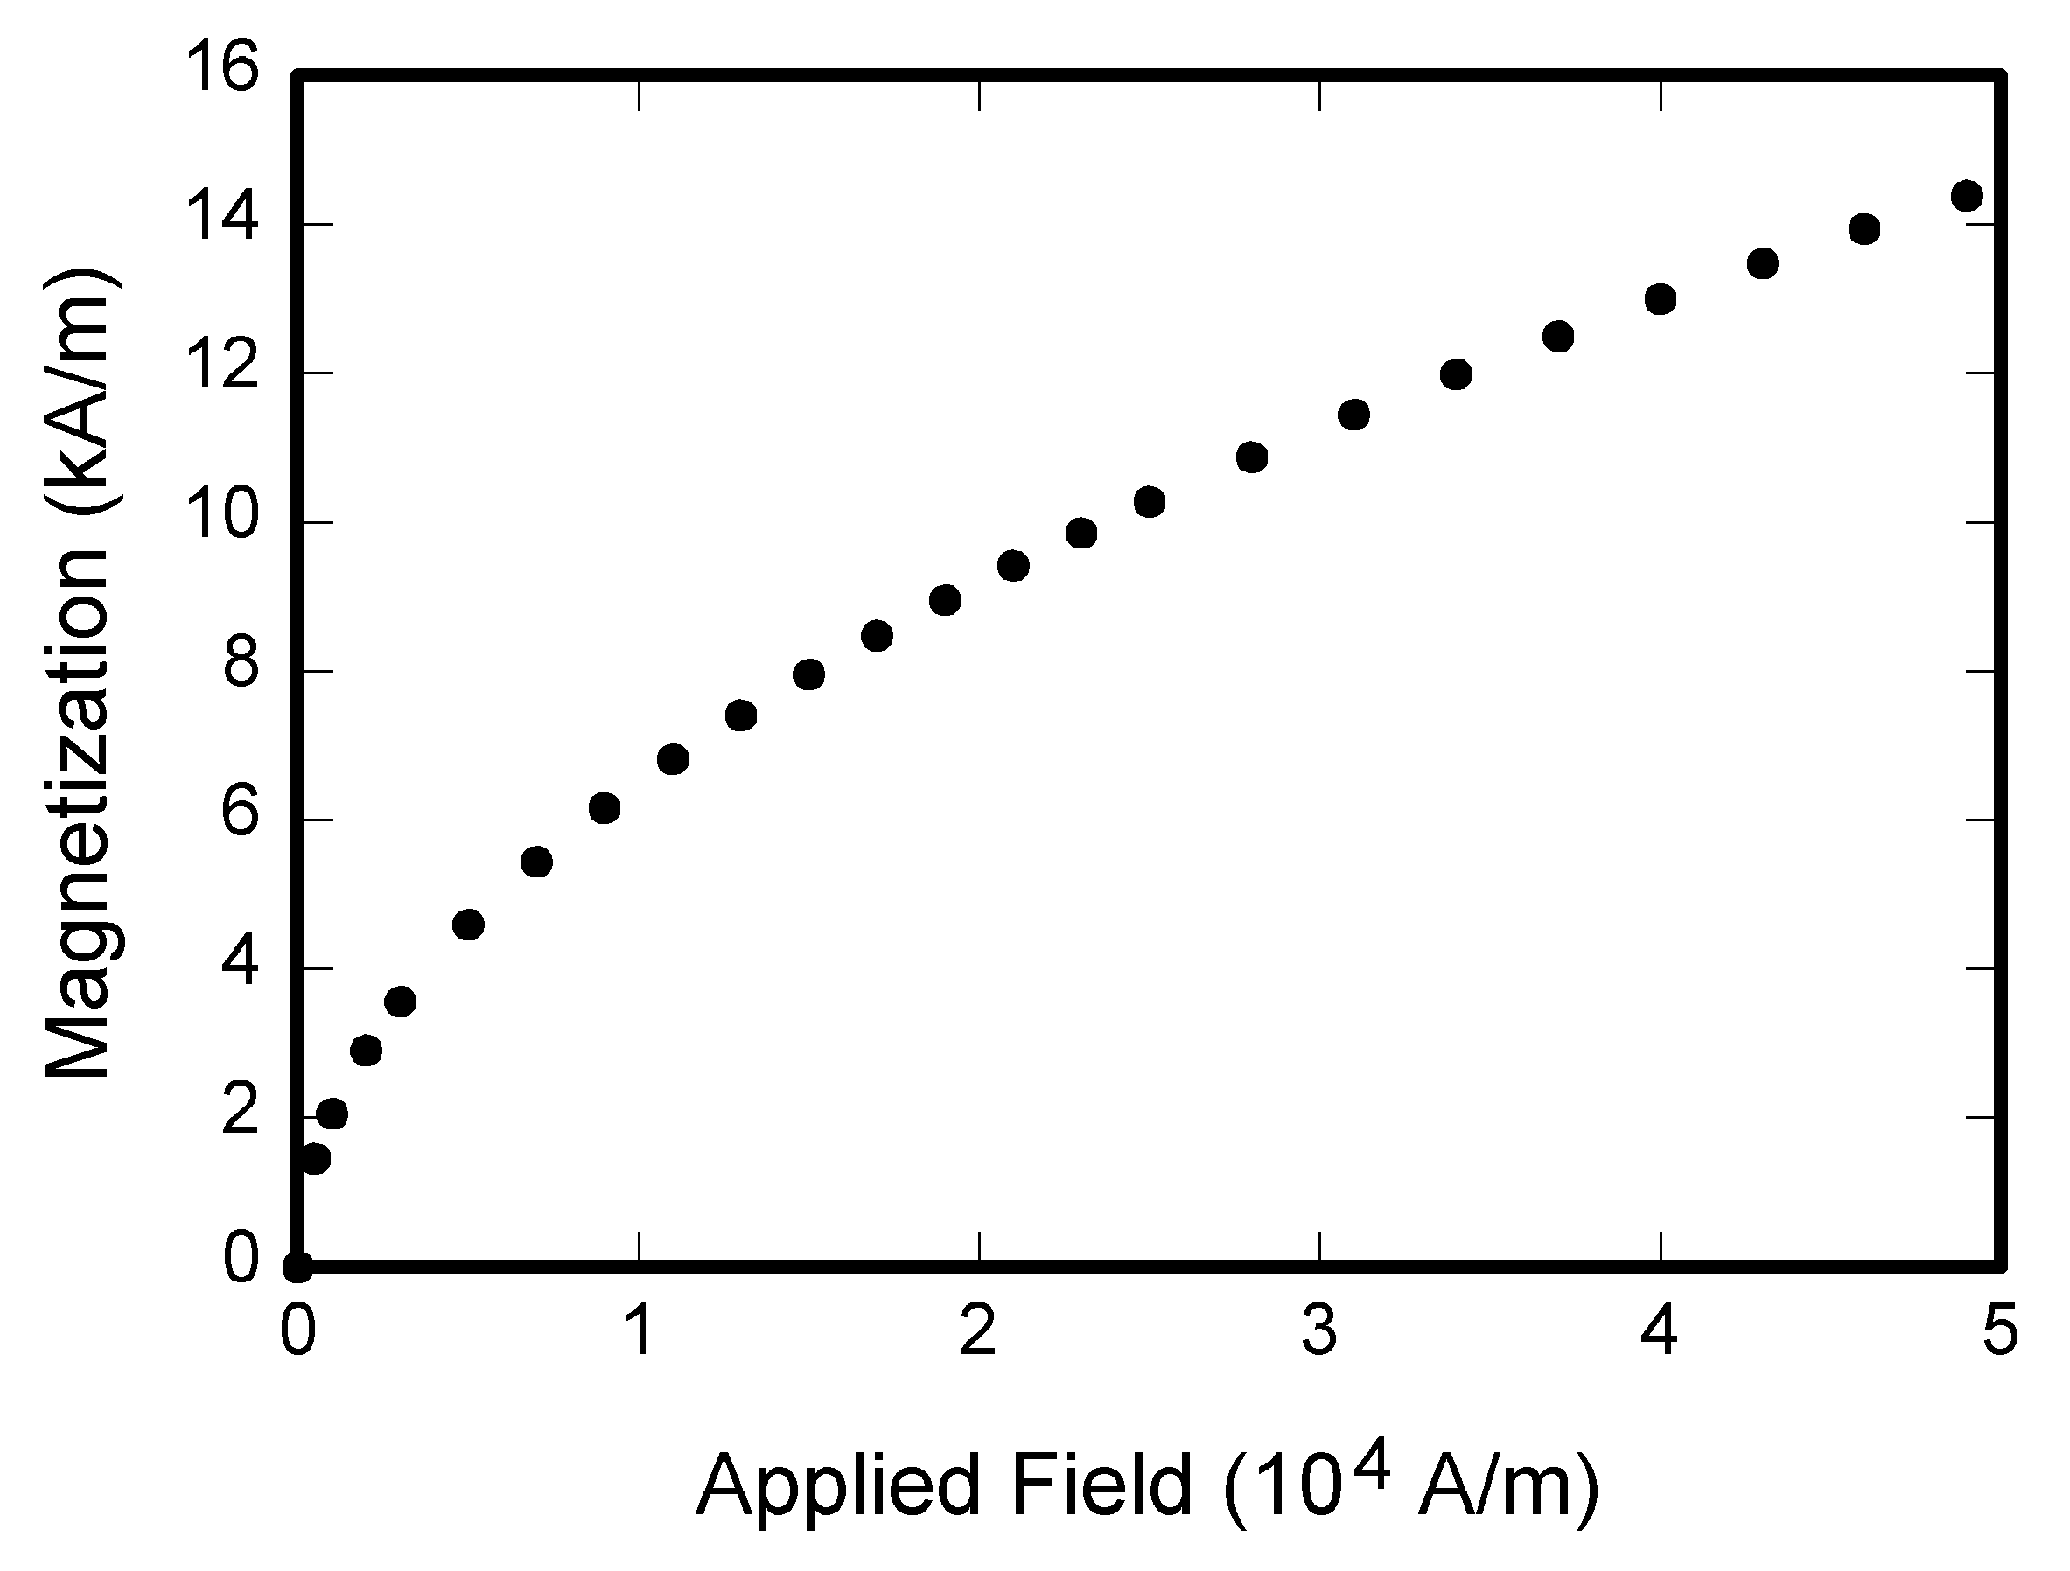
\includegraphics{fig1.png}}
\caption{Example of a figure caption.}
\label{fig}
\end{figure}

Figure Labels: Use 8 point Times New Roman for Figure labels. Use words 
rather than symbols or abbreviations when writing Figure axis labels to 
avoid confusing the reader. As an example, write the quantity 
``Magnetization'', or ``Magnetization, M'', not just ``M''. If including 
units in the label, present them within parentheses. Do not label axes only 
with units. In the example, write ``Magnetization (A/m)'' or ``Magnetization 
\{A[m(1)]\}'', not just ``A/m''. Do not label axes with a ratio of 
quantities and units. For example, write ``Temperature (K)'', not 
``Temperature/K''.




\begin{thebibliography}{00}
\bibitem{b1} A. Glassner, ``An Introduction to Ray Tracing,'' Morgan Kaufmann, 1989.

\bibitem{ericm} E. Lengyel, ``Mathematics for 3D game programming and computer graphics,'' Cengage Course Technology PTR, 2019.

\bibitem{b3} R. Hartley, A. Zisserman, ``Multiple view geometry in computer vision,'' Cambridge University Press, 2004.

\bibitem{kevin} K. Suffern, ``Ray tracing from the ground up,'' CRC Press, 2007.

\bibitem{b5} P. Shirley, R. K. Moreley, ``Realistic ray tracing,'' A K Peters Ltd, 2003.

\bibitem{ericr} E. Lengyel, ``Foundations of game engine development volume 2: Rendering,'' Terathon Software LLC, 2019.

\bibitem{peter} S. Marschner, P. Shirley, ``Fundamentals of computer graphics,'' CRC Press, 2016.

\bibitem{b8} S. J. Gortler, ``Foundations of 3D computer graphics,'' MIT Press, 2012.

\bibitem{b9} M. Ashikmin, P. Shirley, ``An anisotropic Phong light reflection model,'' Technical Report UUCS-00-014, Computer Science Department, University of Utah, 2000.

\bibitem{b10} J. F. Blinn, ``Models of light reflection for computer synthesized pictures,'' Proceedings of SIGGRAPH 77, Computer Graphics, Vol. 11, No. 2, pp. 192–198, 1977.

\bibitem{b11} M. F. Cohen, J. R. Wallace, ``Radiosity and realistic image synthesis,'' Academic Press, San Diego, CA, 1993.

\bibitem{b12} R. L. Cook, K. E. Torrance, ``A reflection model for computer graphics,'' ACM Transactions on Graphics, Vol. 1, No. 1, pp. 7–24, 1982.
\bibitem{cs1} R. L. McFall,and C. A. Cusack , Ray tracing as an object-oriented example for CS 1, The Journal of Computing Sciences in Colleges, 2010, pp.77--84.

\bibitem{pbrt} M. Pharr and G. Humphreys, ``Physically Based Rendering: From Theory to Implementation,'' Morgan Kaufman, 2004.


\bibitem{mycode} A. Raj, ``Very basic ray tracer,'' 2025, gitHub repository. [Online]. Available: https://github.com/induaditya3/computer\_graphics\_ocaml/\\tree/main/ray\_tracer


\bibitem{b16} T. Whitted, ``An improved illumination model for shaded display,'' Communi-
cations of the ACM 23, June 1980.

\bibitem{b17} J. F. Hughes, A. van Dam, M. McGuire, D. F. Sklar, J. D. Foley, S. K. Feiner, K. Akeley, ``Computer graphics: Principles and practice,'' Addison-Wesley, 2013.
\end{thebibliography}

\end{document}
